%---------------------------------------------------------------------------------------------------
%		main.tex
%
%	This is the main file of the chapter that talk about the problem space.
%
%	Author: Andrea Meneghinello
% Version: 0.1
%	Table of changes:
%		15/03/2016 -> document definition
%---------------------------------------------------------------------------------------------------
\chapter{Problem space}
\label{cap:problemSpace}
With this chapter we want to introduce our thesis talking about main problems that developers
encounter during their work. Our focus will be on cloud computing, with special
attention to \ac{paas} level of \ac{spi} cloud model, as a valid solution to relieve their workload.

We will start describing, in Section \ref{sec:problemSpace-useCases}, some use-cases that illustrate
common scenarios and lead us to consider cloud computing model, in Section 
\ref{sec:problemSpace-cloudComputing} as solution for both companies and software-houses. Later we
will focus our attention on the \ac{paas} cloud model, Section \ref{sec:problemSpace-paas}, 
illustrating its main features and characteristics; we also discuss how this cloud model is possible
through virtualization. Progressively we will illustrate Docker, Section
\ref{sec:problemSpace-docker}, a new \acs{os} virtualization level technology that promise to change
the \ac{paas} cloud model; we illustrate its main characteristics, architecture, how it provide
data-management to conclude with a brief digression about the state-of-the-art of security
issues. Finally Section \ref{sec:problemSpace-problem} will give a formal description of the
problem that we will face for the rest of the thesis.

%---------------------------------------------------------------------------------------------------
%		use-cases.tex
%
%	This file contains the sections that describe typical use cases on which we can find the problem
% that will be studied in the master thesis.
%
%	Author: Andrea Meneghinello
% Version: 0.1
%	Table of changes:
%		06/03/2016 -> document definition
%---------------------------------------------------------------------------------------------------
\section{Problem definition}
\label{sec:background-problem}
Nowadays more and more business companies use complex software systems in their daily activities;
from the customer care to internal administration. Until recently, these complex applications are
executed over proprietary hardware systems. This scenario is unfavourable for both companies and
software-houses that have to maintain the applications.

From the companies point of view, in order to keep those applications working, according
to the defined \glossarySng{sla}, they have to invest economic resources in qualified personnel and 
establish complex administration processes. They can solve this problem through the adoption of 
one of the many existent frameworks that allows \acs{it} process management. A well known one is
\keyword{\ac{itil}}. The framework, shown in Figure \ref{img:background-problem-itilProcessModel}, 
defines general best-practices in order to design and instantiate processes that permit a more coherent
administration of \acs{it} departments and the deployed applications. The processes that are relevant
for this problem belong to \ac{sda}. They are  \keyword{\ac{am}} and \keyword{\ac{cm}}. Both processes
focuses on planning and monitoring the effective provision of resources to support all the service
requirements \cite{availabilityCapacityProcesses}.

\begin{figure}
	\centering{}
	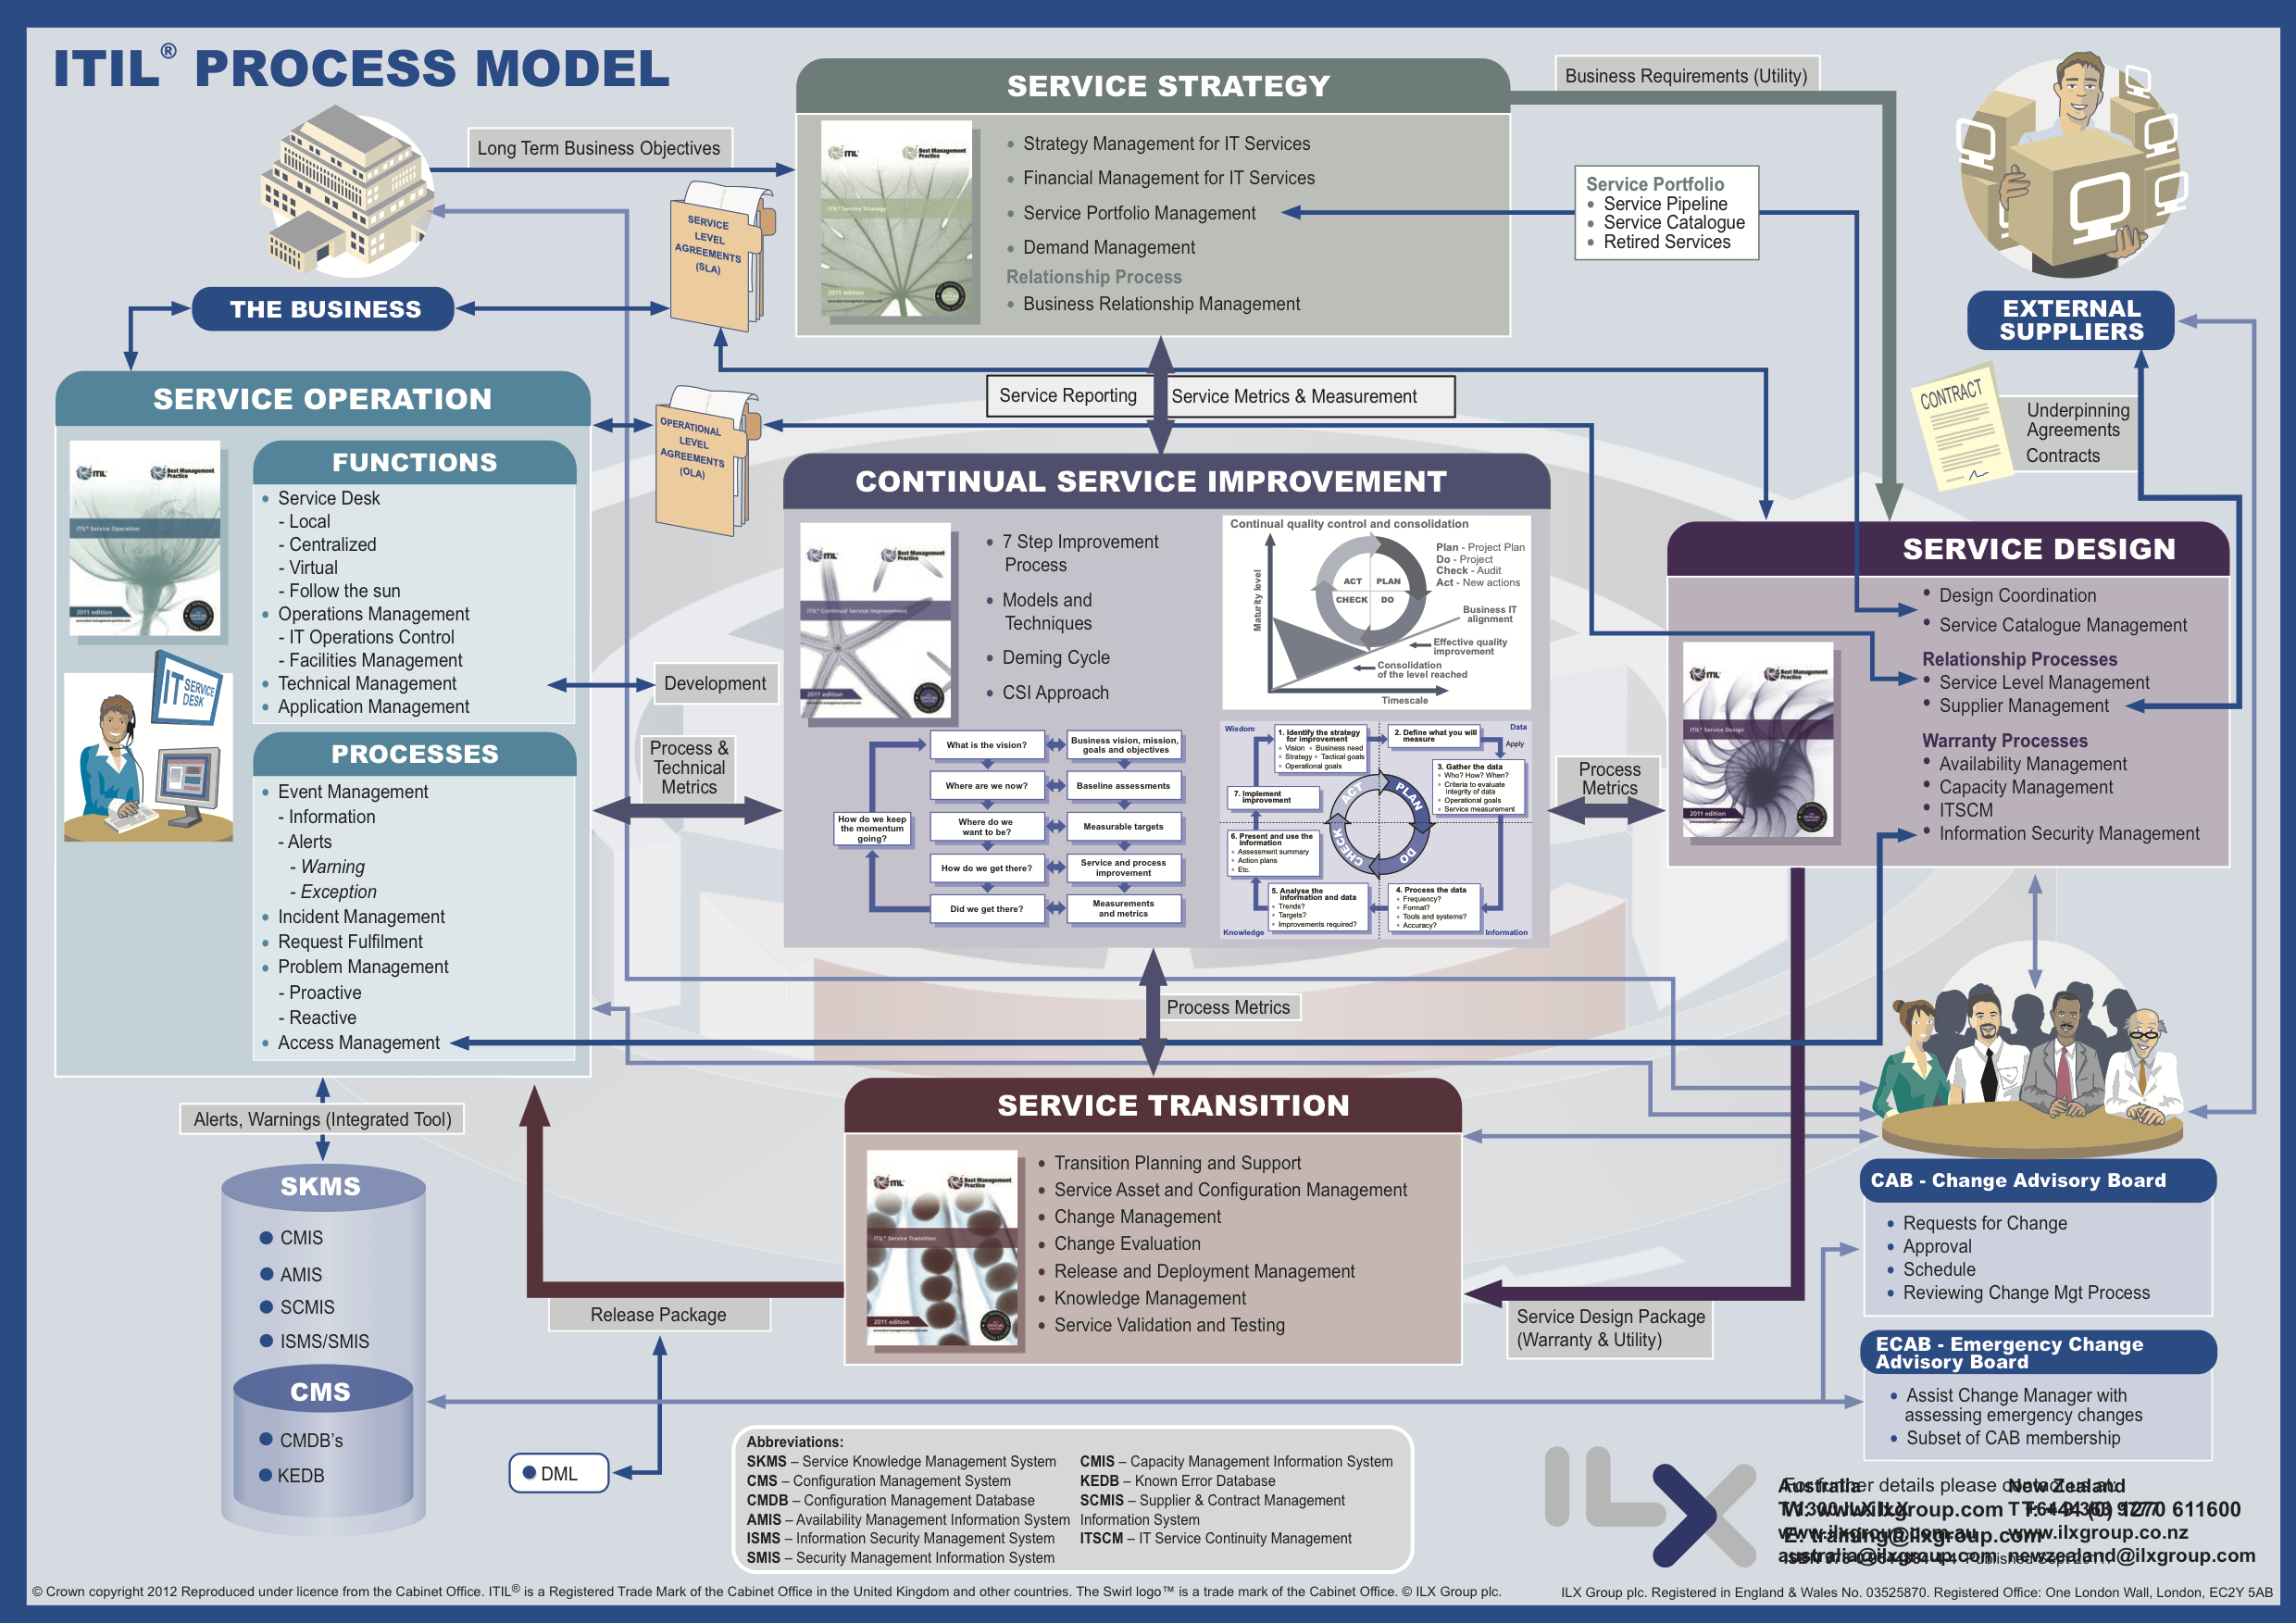
\includegraphics[width=0.8\textwidth]{chapters/background/images/itil-map.png}
	\caption[\acs{itil} v3 process model]{A bird's eye view of the processes defined by the \acf{itil} 
		framework. Their main purpose is to manage software's life-cycle in large business companies
		\cite{itilProcessModel}.}
	\label{img:background-problem-itilProcessModel}
\end{figure}

On the other hand software-houses have to face with different runtime environments (both in term of
hardware and software configurations) which makes the \glossaryPlr{deployment-process} more difficult.
Another problem is represented by unavoidable bug errors that are present in every application. Here
bugs are not only due to development errors but they can be also due to the runtime environment itself.
Thus developers waste a lot of time only to replicate those execution environments, stealing it from
more profitable activities. Finally when the solution is found they have to visit the client to fix
the bugs in loco (if remote assistance is not possible).

Another scenario is the following: software-houses may want to make their software available online
and always up-to-date. End-users should be able to use it anywhere and using any type of device without
any installation process. In addiction they do not have to care about updating that software.

Companies can follow general best-practices to solve the problem. In addiction, many of them have
understood, very well, the benefit of delegating hardware management to cloud providers (see Section
\ref{sec:background-cloudComputing-capexOpex}). Unfortunately, we cannot assert the same things for
software-houses.

Cloud computing is becoming more mature day by day and market has started investing on it. A recent
study, commissioned by Microsoft \cite{microsftCloudNewJob}, shows that cloud computing produces much
new innovation in \acs{it} every year:

\begin{center}
	\begin{quote}
		``Innovation created by cloud computing produce \textdollar{}1.1 trillion a year in new
		business revenues. It was also able to generate 14 million of jobs worldwide from 2011 to 2015.''
	\end{quote}
\end{center}

Therefore, the trend is positive and it is expected to grow more and more in the long term.
Lately, cloud computing model have become a more reliable infrastructure supplier, so companies 
started to earn outsourcing the hardware management. Nevertheless software engineers have to face
again with the construction and the configuration of complex scalable environments, stealing time from
development activities. As a consequence they ask for more automation in building work environments so
they can focus more on development activities (development, test and execution).

We have argued about the major requests made by software developers. Their need for automatic
hardware configuration and ready-to-use work environments promoted the creation of the \ac{paas} 
cloud model. \ac{paas} is one of the three conceptual layers in the \ac{spi} model: \ac{saas} on the
top (faces with end-users); \ac{paas} in the middle (faces with developers) and finally \ac{iaas} on
the bottom where physical resources reside (faces with sysadmins). The \ac{paas} layer is a good place
where managing the elasticity challenges and the related complexity.

%It differs from \ac{iaas} because \ac{paas} does not allow users to control the underlying
%hardware directly. In addiction, it also differs from the \ac{saas} layer because the latter is focused
%on software functionalities while the former is responsible on how the software is deployed and in managing
%the elasticity challenges and the related complexity. 

Despite all \ac{paas} advantages (described in Section \ref{sec:background-paas-characteristics})
the following issues may be still present:

\begin{itemize}
	\item{it may lead to a possible vendor lock-in if the provider imposes the use of a particular
		technology;}
	\item{it may compromise cloud resource elasticity because users are not able to configure the
		underlying hardware resources.}
\end{itemize}

In order for the \ac{paas} vendors to offer high quality services, both for companies and software-houses,
they must provide ready-to-use work environments and key mechanisms that guarantee \keyword{elasticity}
for the deployment units.

Elasticity is one of the key characteristics of the cloud and means that the cloud service can rapidly
scale its dimension according to the clients needs. It can be obtained by the combination of two complementary
dimensions: \keyword{optimization of the \ac{paas} underlying hardware management} and \keyword{specifically
designed software architectures}.

The assets on which the \ac{paas} vendors can make optimizations are those illustrated in Section
\ref{sec:background-virtualization-assets}, hence our contribution is to compare, and then analyse, the
infrastructural costs of both \ac{vm} and Docker based \ac{paas} solutions in terms of computing, storage and
networking.

In addiction we will seek for an architectural pattern that is able to exploit the elasticity mechanisms 
provided by the \ac{paas} layer.

Nowadays cloud computing is able not only to offer unlimited provision of hardware but also the generation
of dynamic work environments. In order to understand how it is possible we must first know what really is
cloud computing and why it is able to help both business companies and software-houses.

%---------------------------------------------------------------------------------------------------
%		cloud.tex
%
%	This file contains the sections of the document that describe the cloud computing.
%
%	Author: Andrea Meneghinello
% Version: 0.1
%	Table of changes:
%		15/03/2016 -> document definition
%---------------------------------------------------------------------------------------------------
\section{Cloud Computing}
\label{sec:problemSpace-cloudComputing}
Cloud computing provides shared resources and data to devices on-demand; providers commonly offer a 
``\keyword{\glossarySng{pay-per-use}}'' model to pay used resources. Hence the pay-per-use model
in \acs{it} is becoming available to the market. It has been proved that it is an effective way to
reduce \acs{it} costs without sacrificing software quality. Consequently the demand for highly
responsive, reactive and cheap \ac{saas}, made by end-users and companies, is increasing (as shown
in Figure \ref{img:problemSpace-cloudComputing-saasInterest}).

%TODO -> controllare se inserire una reference in "It has been proved"
 
\begin{figure}
	\centering{}
 	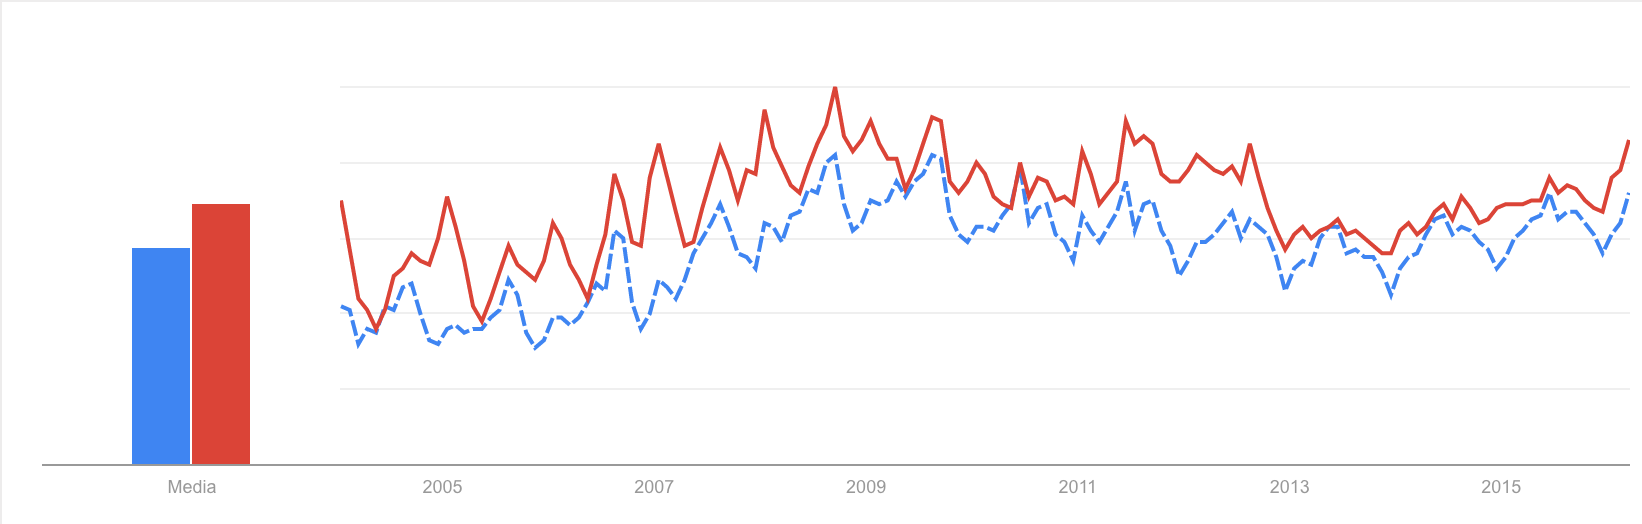
\includegraphics[width=0.75\textwidth]{chapters/problem/images/saas-interest.png}
 	\caption[Trends in searching ``\acs{saas}'' on Google]{\acf{saas} and its acronym (\acs{saas})
 		terms search since 2004 in Google's investigation made all over the world. In red we can see
 		results about ``\acs{saas}'' term search instead in blue we have the ``\acf{saas}'' one. 
 		(\footnotesize{source	Google Trends}\normalsize{)}}
 	\label{img:problemSpace-cloudComputing-saasInterest}
\end{figure}

Cloud computing helps also software-houses, providing them \keyword{ready-to-use work environments}.
This solution makes software-houses save both money and time because developers do not waste time in 
building the work environments on their own. In addiction those work environments are \keyword{elastic},
hence they can build and deploy their application and make them ubiquitous. Therefore the demand for
this particular kind of cloud platform is increasing, as shown in Figure
\ref{img:problemSpace-cloudComputing-paasInterest}.

\begin{figure}
	\centering{}
	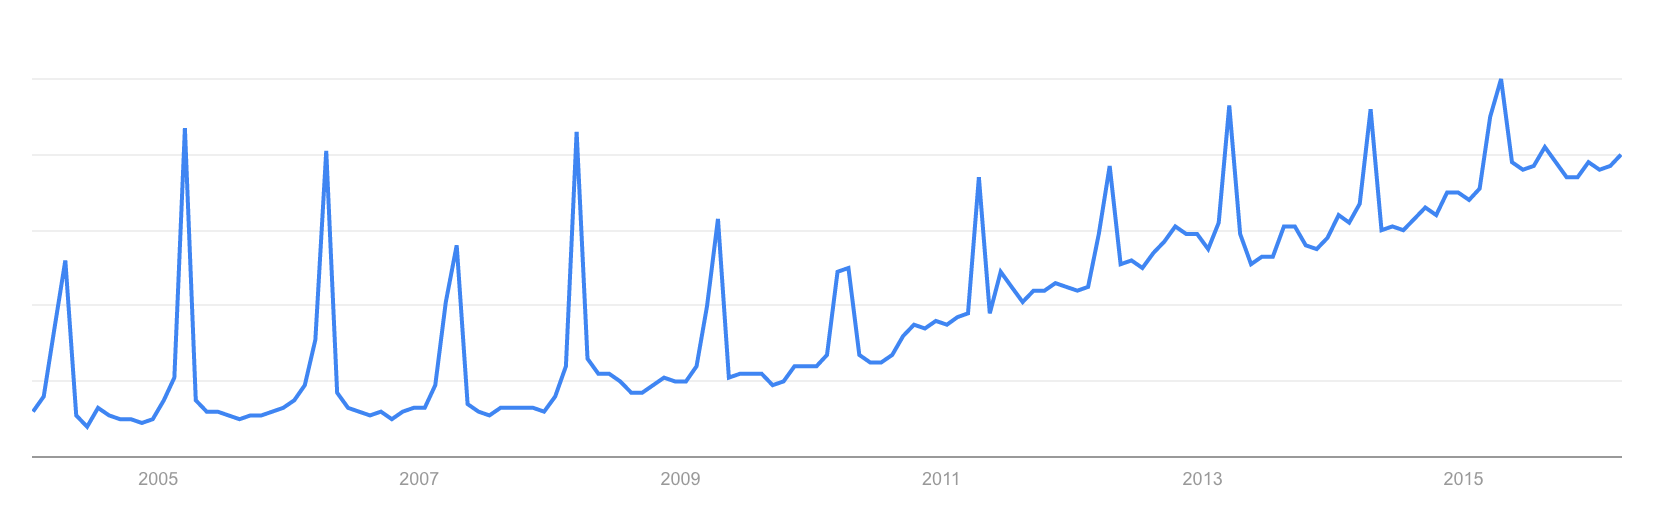
\includegraphics[width=0.75\textwidth]{chapters/problem/images/paas-interest.png}
	\caption[Trends in searching ``\acs{paas}'' on Google]{\acf{paas} terms search since 2004 in Google's
		investigation made all over the world. (\footnotesize{source	Google Trends}\normalsize{)}}
	\label{img:problemSpace-cloudComputing-paasInterest}
\end{figure}

To make their software exploit the elasticity offered by cloud environments, software-houses need to redesign
them using appropriate architectural patterns. Before discussing about those patterns, it is necessary to do a
brief digression about what cloud computing really is and why in the nearly future many more companies and
software-house will start a migration to it.

The most comprehensive definition of what cloud computing is comes from \ac{nist} in \cite{nistCloudComputing}:

\begin{center}
	\begin{quote}
		\textit{``a model for enabling ubiquitous, convenient, on-demand network access
			to a shared pool of configurable computing resources that can be rapidly provisioned and released
			with minimal management effort or \acf{sp} interaction."}
	\end{quote}
\end{center}

In following Sections we will show, in details, the benefits of its adoption by presenting its main
characteristics.

\subsection*{Moving from platform ownership to platform management}
\label{sec:problemSpace-capexOpex}
When companies decide to design, and consequently build, a new software service they have to plan how
many resources (compute capacity, storage and networking) making available in order to respect the defined
\ac{sla}. Developers have to build, over the provisioned resources, the working environment to build
and support the application.

This leads to predict the worst possible cases and to invest in resources that permit to cope this
situation as well as find a business grow model that maintains enough availability without weighing
too much on the investments. Even if this prediction is able to detect the worst cases it imposes
large capital investments and heavy fixed costs on firms, which lead to redundant expenditures and
high level of overcapacity, both in term of technology and in term of qualified personnel in its
management. The cited business model is known with the name of \keyword{\ac{capex}}.

Opposite to the \ac{capex} business model there is the \keyword{\ac{opex}}. This is more flexible
because it does not require to invest in capital ownership (hardware and time to build the work
environment) but instead in renting both the desired amount of resources and the ready-to-use work
environments and simply release them when they are no more necessary. This model, if correctly applied,
permits a cost reduction; Figure \ref{img:problemSpace-capexOpex-model} shows a chart which compares
both models. We can also see that there will be a moment (in the adoption of \ac{capex} one) on which
there is a lack in the available resources leading to a decline of the service and to a possible \ac{sla}
violation.

\begin{figure}
	\centering{}
	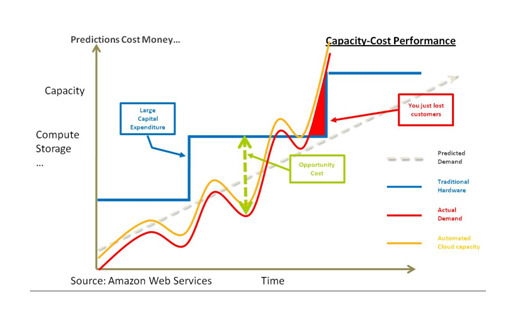
\includegraphics[width=0.9\textwidth]{chapters/problem/images/capex-opex.png}
	\caption[Comparison between \acs{capex} and \acs{opex} business models]{Comparison of \acf{capex}
		and \acf{opex} business models.}
	\label{img:problemSpace-capexOpex-model}
\end{figure}

We can observe these two different business models also in two real case scenarios \cite{netflixZynga}
that involve two well known software houses, in the world of mobile/social-network games and the other
in video content sharing: they are \textit{Zynga} and \textit{Netflix}. 

The most famous product of Zynga is \textit{Farmville}. It was released in 2009 and became, in a very
short period, very popular between Facebook users (it reached 10 million of active users in less than
6 weeks). Initially the service was hosted inside the Amazon infrastructure but two years later his
\acs{ceo}, Frank D. Gibeau, decided to invest \textdollar{}100 million to build a proprietary data-centre
to host the service assuming to obtain a long term cost reduction. In Figure
\ref{img:problemSpace-capexOpex-zyngaCase} we can see the trend of \ac{mau} of Farmville application
in the months that follow the opening of new data-centre. It is possible to observe that \ac{mau} reached
its peak in 2012 (when the new centre became operative) but in the following two years this value had
been divided by three (as the new infrastructure demanded), leading to consistent economic losses.
Thus the society has decided to return basing its service on the Amazon Infrastructure.

\begin{figure}
	\centering{}
	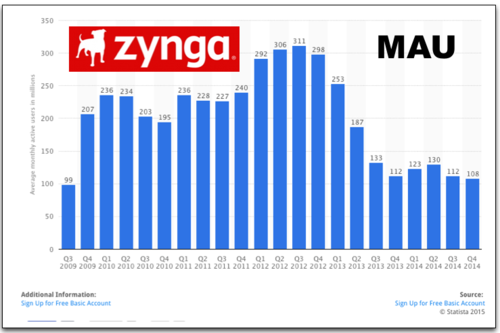
\includegraphics[width=0.6\textwidth]{chapters/problem/images/zynga-case.png}
	\caption[\acs{mau} of Farmville application after 2012]{\acf{mau} of the Farmville application from
		2012 when company decide to invest in a proprietary data-centre. We can observe that after two
		years the users' demand is divided by three as the infrastructure demand \cite{netflixZynga}.}
	\label{img:problemSpace-capexOpex-zyngaCase}
\end{figure}

Netflix, born in 1997 with a rent \acs{dvd} service, started a new \ac{vod} business in 2007 and, as
in the case of Zynga, chose to base its new business on the Amazon infrastructure. The most relevant
difference is that Netflix never chose to change its infrastructure supplier when it saw that his
business was starting to succeed. This choice allowed Netflix to become the major \ac{vod} competitor.

\subsection*{Cloud Computing key characteristics}
Taking as a reference the \ac{nist} definition of cloud computing \cite{nistCloudComputing}, a pool of resources
must offer the following characteristics (shown in Figure \ref{img:problemSpace-cloudComputing-characteristics})
to the end-users to be considered a cloud environment:

\begin{itemize}
	\item{\keyword{on-demand self-service}: refers to way on which people can procure resources, specifically
		they should be made available to users on-demand with automatic procedures;}
	\item{\keyword{broad network access}: refers to the way on which people can get them; a cloud provider
		must not restrict the access to them by imposing the use of a particular technology;}
	\item{\keyword{resource pooling}: refers on the way on which the cloud provider makes them available to
		customers; it must make them accessible as a single and compact set of resources even if the are
		distributed on many servers inside the data-centre;}
	\item{\keyword{rapid elasticity}: refers on the way on which resources can be provisioned and released
		to maintain the software highly available while keeping the monthly/hour\footnote{Usually we have a
		monthly rent in case of adoption of \acs{paas} cloud model, instead we have a hour rent if we adopt
		a \acs{iaas} cloud model. We illustrate the difference in following sections.} rent as low as possible;}
	\item{\keyword{measured service}: refers on the way on which both the end-user and the cloud provider
		can measure the resource consumption. This is fundamental for final users to know the total amount of
		the rent and for cloud provider to keep under control resource consumption and scale them only when
		it is really necessary.}
\end{itemize}

\begin{figure}
	\centering{}
	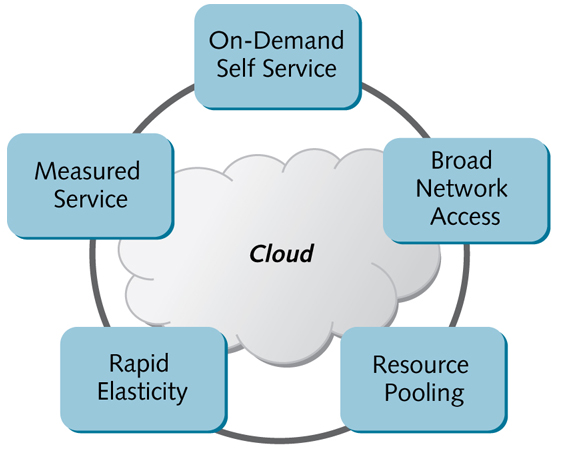
\includegraphics[width=0.5\textwidth]{chapters/problem/images/cloud-characteristics.png}
	\caption[Key characteristics of cloud computing]{An overview of the five characteristics that makes a
		pool of shared resources a cloud computing environment \cite{cloudCharacteristics}.}
	\label{img:problemSpace-cloudComputing-characteristics}
\end{figure}

\subsection*{Available service models}
\label{sec:problemSpace-cloudServiceModels}
Nowadays cloud computing makes available many service models (shown in Figure
\ref{img:problemSpace-cloudComputing-serviceModels}):

\begin{itemize}
	\item{\keyword{\acf{saas}}: the capability provided to the end-user is to use the provider's
		applications running on a \glossarySng{cloudInfrastructure}. Programs are accessible from various
		client devices through either a thin interface, such as a web browser (e.g. web-based e-mail),
		or a program interface. The user does not manage or control the underlying cloud infrastructure
		including network, servers, operating systems, storage, or even individual application capabilities,
		with possible exception of limited user specific application's configuration settings;}
	\item{\keyword{\acf{paas}/\ac{caas}}: the capability provided to the end-user is to deploy onto the cloud
		infrastructure user-created or acquired applications created using programming languages,
		libraries, services and tools supported by the provider.\footnote{This capability does not preclude
		use of compatible tools like other sources.} The user does not manage or control the underlying
		cloud Infrastructure including network, servers, operating systems or storage, but has control
		over the deployed applications and possibly configuration settings for the application-hosting
		environment;}
	\item{\keyword{\acf{iaas}}: the capability provided to the end-user is to provision processing, storage,
		network and other fundamental computing resources where the consumer is able to deploy and run
		arbitrary software, which can include \acs{os} and applications. The final user does not
		manage the underlying cloud infrastructure but has control over operating systems, storage, and
		deployed applications; and possibly a limited control of selected networking components (such as
		network firewall).}
\end{itemize}

To help to understand how these three components are related together, Randy Bias \cite{differenceIaasPaas}
create this transportation analogy:

\begin{quote}
	``By itself, infrastructure is not useful. It just sits there waiting for someone to make it productive in
	solving a particular problem. Imagine the Interstate transportation system in the \acs{us} Even with all
	these roads built, they would not be useful without cars and trucks to transport people and goods. In this
	analogy, the roads are the infrastructure and the cars and trucks are the platform that sits on top of the
	infrastructure and transports the people and goods. These goods and people might be considered the software
	and information in the technical realm''.
\end{quote}

\begin{figure}
	\centering{}
	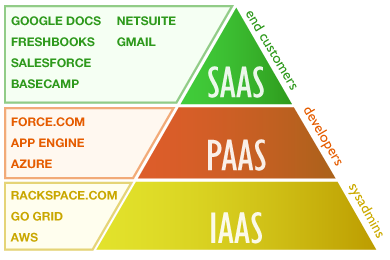
\includegraphics[width=0.55\textwidth]{chapters/problem/images/cloud-service-models.png}
	\caption[Available service models in cloud computing]{An overview of available cloud service models. On the
		left we can observe example of ``environments'' that uses the specified models, while on the right we
		have the people interested for that specific models \cite{cloudServiceModels}.}
	\label{img:problemSpace-cloudComputing-serviceModels}
\end{figure}

\subsection*{Available deployment models}
\label{sec:problemSpace-cloudDepoymentModels}
Cloud Computing can assume different forms:

\begin{itemize}
	\item{\keyword{Private Cloud}: the cloud infrastructure is provisioned and used by a single organization
		comprising multiple customers (e.g. business units). It may be owned, managed and operated by the
		organization, a third party or some combination of them and it may exist on or off premises;}
	\item{\keyword{Community Cloud}: the cloud infrastructure is provisioned for exclusive use by a specific
		community of users from organizations that have shared concerns (e.g. mission, security requirements,
		policy, and compliance considerations). It may be owned, managed and operated by one or more of
		the organizations in the community, a third party or some combination of them, and it may exist on
		or off premises;}
	\item{\keyword{Public Cloud}: the cloud infrastructure is provisioned for open use by the general
		public. It may be owned, managed and operated by a business, academic, government organization or
		some combination of them, and it may exist on or off premises;}
	\item{\keyword{Hybrid Cloud}: the cloud infrastructure is a composition of two or more distinct
		cloud infrastructures (private, community or public) that remain unique entities, but are bound
		together by standardized or proprietary technology that enables data and application portability
		(e.g. cloud bursting for load balancing between clouds).}
\end{itemize}

\subsection*{Isolation and resource control}
\label{sec:problemSpace-cloudComputing-isolationResource}
With the adoption of cloud computing, software-houses have isolation between hardware management and the software
development that makes possible to separate the work of hardware engineers and software developers.
Now it is possible to maintain the hardware updated without worrying about the software. For example Amazon
System Engineers can decide to upgrade the storage hardware from the magnetic to solid state technology without
informing software-houses or users, that have applications deployed on it. On the other hand software-houses
and users do not need to alter and/or redeploy software after the change occurred. Often these changes are
transparent to the final users. 

However the introduction of cloud computing introduces a series of new problems that software developers must
master to develop high productive software. One critical issue that occurred when companies has began to use cloud 
computing is that they started to share a common base: the hardware on which the software executes.

\keyword{Isolation} and \keyword{resource control} have become two critical requirements when we are co-locating
applications of different companies in the same cloud computing environment. Isolation refers to the requirement
that execution of one software must not affect the execution of another one in the same system. Resource control
instead refers to the ability to constrain software execution to a specific set of resources.

In cloud settings, while performance isolation is desirable, it is often secondary to functional and security
isolation wherein one software cannot learn anything or affect the correctness of another one. Memory capacity
and compute capability are two levers in resource control through which a software is constrained to consume
no more than a certain amount of memory capacity and execute no more than a certain number of cores.

%---------------------------------------------------------------------------------------------------
%		paas.tex
%
%	This is the main file of the chapter that talk about the paas layer of SPI.
%
%	Author: Andrea Meneghinello
% Version: 0.1
%	Table of changes:
%		15/03/2016 -> document definition
%---------------------------------------------------------------------------------------------------
\section{\acf{paas}}
\label{sec:background-paas}
In the remaining of the thesis our focus will be on the \keyword{\ac{paas}} service model.
\ac{paas} is like a \glossarySng{middleware}. It is a set of services that helps developers
to develop and test software without having to worry about provisioning servers, storage and backup
associated with developing and launching a new service. Developers want to write code, test the service,
launch it and be able to continually make changes to it to fix bugs. All the back-end issues about setting
up servers should be done automatically and transparently in background.

\ac{paas} and middleware are not the same thing. The main purpose of middleware is to offer
sophisticated features to developers, such as: transactions, security, clustering, etc. These features
allow them to build their custom applications instead of solving those hard problems repeatedly.
However middleware is only ``static'' software meaning that it must be configured, deployed and
administrated on servers by qualified personnel. All those tasks are usually assigned to \acs{it} teams.
Instead \ac{paas} is a superset of middleware and offers all these good features to developers
in addition to covering the operational aspects that where typically owned by \acs{it} teams.

Figure \ref{img:background-paas-spiResponsibilities} illustrates, in a transparent way, what are the
developers responsibility in the different stacks which compose the \ac{spi} model. We can see that
if we adopt the \ac{paas} model, we are only responsible for our code and its data.

\begin{figure}
	\centering{}
	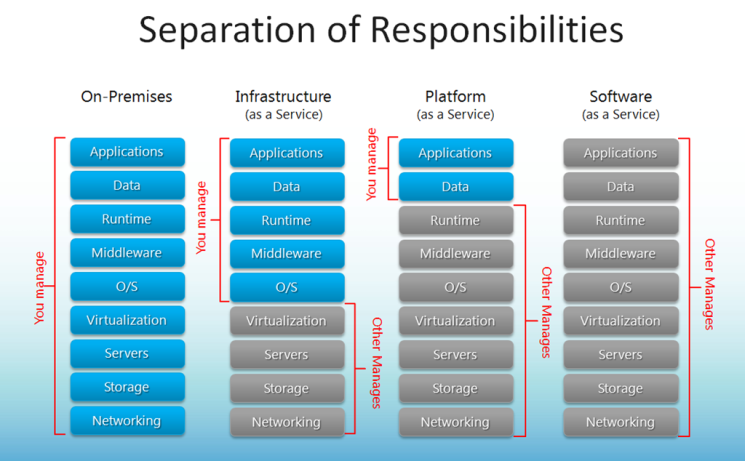
\includegraphics[width=0.8\textwidth]{chapters/background/images/separation-responsabilities.png}
	\caption[Separation of responsability in \acs{spi}]{Separation of responsability in different stacks
		of the \acf{spi} model compared with the on premises one \cite{spiRepsonabilities}.}
	\label{img:background-paas-spiResponsibilities}
\end{figure}

As we argued in Section \ref{sec:background-cloudComputing-cloudDepoymentModels}, \ac{paas} is possible
because is ``sitting'' over the \ac{iaas} infrastructure and through virtualization is able to provide many
features to developers. In following sections we will deep the concept of \ac{paas}
analysing its main characteristics and and the scenarios in which it is mostly useful and where it may not
be the best option. 

Later, in Section \ref{sec:background-virtualization} and \ref{sec:background-docker}, we will respectively
describe virtualization technique and containerization with Docker because they are used to ``build''
the software deployment units managed by the \ac{paas} level.

\subsection{Main characteristics}
\label{sec:background-paas-characteristics}
\ac{paas} offers to developers the following basic characteristics:

\begin{itemize}
	\item{it is able to maintain, inside the same \ac{ide}, services to develop, test and deploy
		applications;}
	\item{web based \ac{ui} creation tools help to create, modify, test and deploy different \ac{ui}
		scenarios;}
	\item{it makes possible multi-tenant architectures where multiple concurrent users utilize the same
		development application;}
	\begin{itemize}
		\item{support for development team collaboration: some \ac{paas} solutions can include project
			planning and communication tools;}
	\end{itemize}
	\item{it makes possible multi-tenant architectures where multiple concurrent users utilize the same
		deployed application\footnote{The application must be designed to support multiple concurrent
			users.};}
	\item{built in scalability of deployed software including load balancing and fault-tolerance;}
	\item{integration with databases and web services via common standards;}
	\item{tool to handle billing and subscription management.}
\end{itemize}

\ac{paas} is similar in many ways to \ac{iaas} but differentiate from it by the addition of value added
services and comes in two various types:

\begin{itemize}
	\item{a collaborative platform for software development, focused on workflow management regardless
		of the data source being used for the application. An example of this approach is Heroku, a
		\ac{paas} that utilizes Ruby on Rails language;}
	\item{a platform that allows for the creation of software that utilizing proprietary data from an
		application. This sort of \ac{paas} can be seen as a method to create applications with a common
		data form or type. An example is the Force.com from Salesforce.com which is used almost exclusively
		to develop applications that work with the Salesforce.com \ac{crm} tools.}
\end{itemize}

\ac{paas} owns the aforementioned characteristics because exploit better the feature that \ac{iaas}
is able to provide though virtualization. In the next section we will deep the concept of virtualization
to get to present the \acs{os} level of virtualization that cover a relevant part of this thesis.

\subsection{Where it makes sense}
\label{sec:background-paas-whereToUse}
\ac{paas} is very useful in any situation where multiple developers work on a development project or
where other external parties need to interact with the development process. As the case study illustrated
below, it is proving invaluable for those who have an existing data source, for example sales information
from a \ac{crm} tool, and want to create applications which leverage that data. Finally \ac{paas} is useful
where developers wish to automate testing and deployment services.

The popularity of \glossarySng{agile} will also increase the uptake of \ac{paas} as it eases the
difficulties around rapid development and iteration of software.

Some examples of \ac{paas} include \ac{gae} \cite{googleAppEngine}, Microsoft Windows Azure
\cite{windowsAzure} and finally Salesforce.com \cite{salesforcePlatform}.

\subsection{Where it may not be the best option}
\label{sec:background-paas-whereNotToUse}
There are many positive aspects that bring us adopting \ac{paas}, but there also some scenarios where it
may not be ideal. Examples include:

\begin{itemize}
	\item{where the applications need to be highly portable\footnote{In terms of where they are hosted.};}
	\item{where proprietary languages or approaches would impact on the development process;}
	\item{where a proprietary language would hinder later moves to others provides. Concerns are raised
		about vendor lock-in \cite{vendorLockin};}
	\item{where application performance requires customization of the underlying hardware and/or software.}
\end{itemize}

\subsection{A case study}
\label{sec:background-paas-caseStudy}
Menumate \cite{menumateCaseStudy} is a provider of point of sale hardware and software for the hospitality
industry across Australasia. It has taken advantage of the Force.com \ac{paas} to migrate over time a
series of legacy applications used in the business.

Trineo's \cite{trineoCaseStudy} directors of development explained that the use of Force.com platform has
allowed Menumate to centralise, modernise and integrate an otherwise disparate in-house software toolkit. 
They also asserted that a more conventional development approach would require significant infrastructure,
connectivity, security; this also would introduce uptime considerations. Instead the Force.com
platform inherently provides these non-functional requirements, allowing both Menumate and Trineo to
focus purely on developing the needed functionality. Additionally, utilizing a \ac{paas} approach
has meant Trineo could take advantage of both existing integration and deployment tools.

Utilizing a \ac{paas} development environment has resulted in the creation of applications being
significantly faster than would otherwise be the case. In absence of \ac{paas}, the cost of developing
applications would be prohibitive for many companies.

%---------------------------------------------------------------------------------------------------
%		docker.tex
%
%	This file contains the sections that describe the Docker project and its architecture
% models
%
%	Author: Andrea Meneghinello
% Version: 0.1
%	Table of changes:
%		12/03/2016 -> document definition
%---------------------------------------------------------------------------------------------------
\section{Docker containers}
\label{sec:background-docker}
Docker started its life as an open-source project at “dotCloud”, a cloud-centric PaaS company, in early
2013.

Initially Docker was the natural extension of the technology that company had developed to run its cloud
business on thousands of servers. It was written in Go, a statically typed programmed language developed
by Google with syntax loosely based on C. In the next months the company, having regard to the obtained
results, joined the Linux Foundation and changed its name to Docker Inc. and announced that was shifting
its focus on the development of Docker and its ecosystem.

Docker is an open platform for developing, shipping and running applications, it is designed to deliver
software as faster as possible thanks to a shorter cycle between writing and running code. It allows the
separation of the application from the infrastructure and treats the last one like a managed application.
It allows this combining a lightweight container virtualization platform with workflows and tools
that help in managing and deploying applications.

In its core, Docker provides a way to run almost any application securely isolated in a container.
Isolation and security allow to run many containers simultaneously on the same host. Its lightweight
nature, which run without the extra load of a hypervisor, means that we can get more out from the
hardware.

Tools and a platform surround containers so they can help in several tasks:

\begin{itemize}
	\item{getting applications (and supporting components) into containers;}
	\item{distributing and shipping containers to different teams for further development and testing;}
	\item{deploying applications to production environment, whether it is in local data-centre or in the
		cloud.}
\end{itemize}

In the following sections we will discuss about its architecture, and how it is able to manage users'
data and resolve the dependency-hell problem. Finally we will do brief a digression about the state-of-art
in security.

\subsection{Docker architecture}
\label{sec:background-docker-architecture}
Docker is based on a client-server architecture: the \keyword{client} and \keyword{daemon}. Docker
client ``talks'' with the daemon, which does the hardest work of building, running and distributing
the containers. Users cannot directly interact with the daemon: they must write commands for it 
through the client.

Both the Docker client and the daemon can run on the same system, or it is possible to connect the
first one to a remote daemon. They can communicate via sockets or through a RESTful \acs{api}.

The Docker ecosystem, shown in Figure \ref{img:background-docker-architecture-architecture}, is
composed by the following components: \keyword{images}, \keyword{registries} and finally
\keyword{containers}.

\begin{figure}
	\centering{}
	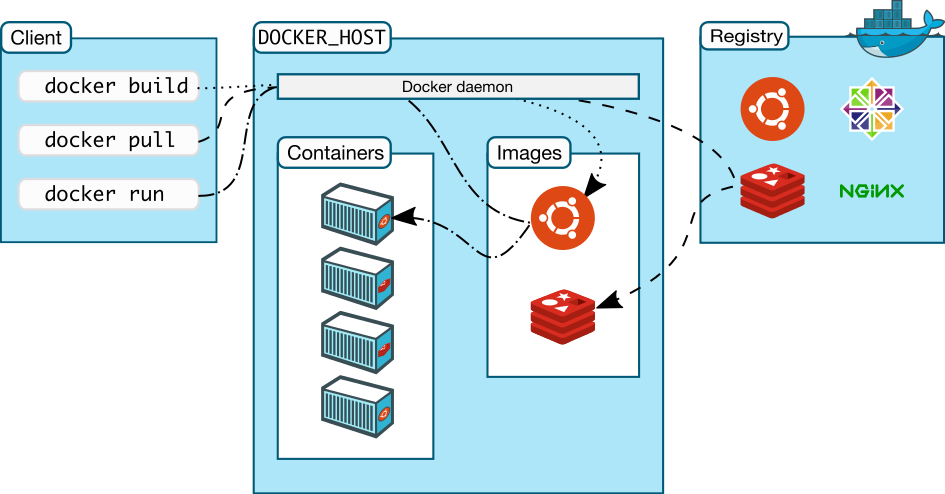
\includegraphics[width=0.8\textwidth]{chapters/background/images/docker-architecture.png}
	\caption[Docker architecture overview]{Docker architecture overview. We can see that a command
		received by the Docker client is forwarded to the Docker daemon which manages the container
		life-cycle. To the right there is the registry that holds the published images.}
	\label{img:background-docker-architecture-architecture}
\end{figure}

A Docker image is a read-only template that Docker uses to create the runnable container; it provides
a simple way to build new images or to update existing ones. A Docker image is created defining a
file (called dockerfile), that contains a description of the application/service (and its dependencies)
that will be contained when it runs. Each image consists of a series of layers; they are combined together
into a single and compact image thanks to the use of \ac{ufs}\footnote{We will discuss about \ac{ufs}
afterwards when we will cover how data are managed.}. Docker images are the build component of the
Docker ecosystem.

Docker registries hold images; these can be public or private stores from which we can upload or
download images. The most famous public registry is provided by Docker and it is called Docker Hub, while
private ones are created and maintained by private companies for proprietary use. Registries serve a
huge collection of existing ready-to-use images. They are the distribution component of the Docker
ecosystem.

Finally Docker containers are an isolated and secure application platform, similar to a system directory
that holds everything that is needed by the application to run. When users decide to deploy a new
container, they make a request to the Docker client; the client forwards the request to the Docker
daemon, which reads the corresponding image and uses it to “give life” to the container. Docker containers
can be run, started, stopped, moved, and deleted easily. They are the run component of the Docker ecosystem.

With Docker containers we can achieve isolation and resource control (important features of SaaS)
through the use of namespaces and cgroups (see Section \ref{sec:background-virtualization-types})

To manage isolation and resource control, Docker largely uses Linux-kernel features, but different kernels
can have contrasting interfaces for the same functionalities. This is the reason why Docker, since v0.9,
replaced the old \ac{lxc} execution environment (which contains cgroups and namespaces) with
\keyword{LibContainer} (shown in Figure \ref{img:background-docker-architecture-libcontainer}).

\begin{figure}
	\centering{}
	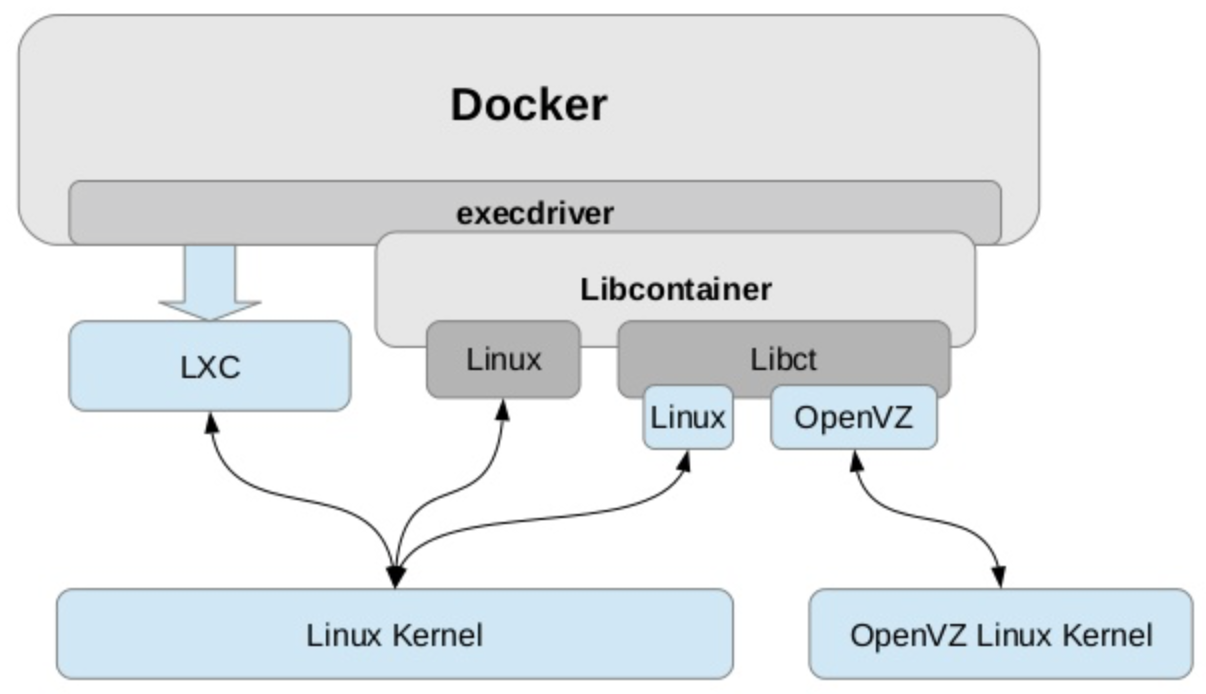
\includegraphics[width=0.6\textwidth]{chapters/background/images/libcontainer.png}
	\caption[Docker libcontainer overview]{Now Docker execution environment is separated from the underlying
		\acs{os} though the introduction of LibContainers.}
	\label{img:background-docker-architecture-libcontainer}
\end{figure}

LibContainer is now the default Docker execution environment. It is meant to be a cross-system abstraction
layer being an attempt to standardize the way applications are packed up, delivered and run in isolation.
Thus, container features available in Linux kernel \acs{api} are provided as a unique library in a
consistent way; it addresses the problem of having an unique kernel \acs{api} and several implementations.

LibContainer has become a stand alone project, after Docker decided to donate it to the open-source community,
therefore other developers (Google, Parallels, RedHat, Ubuntu and others) can contribute to improve its development.

As we just stated, Docker containers are executed in isolation, but this do not prevent them to share data using
the network. Containers can be connected together in two different ways: through a connection based on 
IP-address/TCP-port or the link feature.

In the first case containers, that have an unique IP address, must open outward a TCP port on which they can
listen for incoming connections. Even if it seems reasonable using this type of network connection to share
data, this can instead lead to security problems because connections can arrive also from the web. On the other
hand establishing a connection, between containers, through the link feature is like building a \ac{vpn};
which means less risks for the safety factor, because the connection is only available between different
containers behind the same firewall\footnote{We will analyse in Chapter REF the benefit of this feature.}.

\subsection{Data management}
\label{sec:background-docker-dataManagement}
Docker images are read-only templates from which Docker containers are lunched. Each image consists of
a series of layers combined into a single image using the \acf{ufs} technology.

One reason why Docker is lightweight derives from these layers. When a developer changes a Docker image,
e.g. to deploy a new version of an application, a new layer is built. Thus, rather than replacing
or entirely rebuilding the whole image, as in case of \ac{vm}s, only that layer is added or updated thus
making the Docker image distribution faster and simpler; just this one will be distributed.

\ac{ufs} (shown in Figure 6) is a stackable \ac{fs} which implements the union-mount features. That allows
to specify a series of different \ac{fs} (called branches) which are finally presented as a virtual
and coherent one, even though the branches come from different \ac{fs}. This process is commonly
referred to as namespaces unification.

\begin{figure}
	\centering{}
	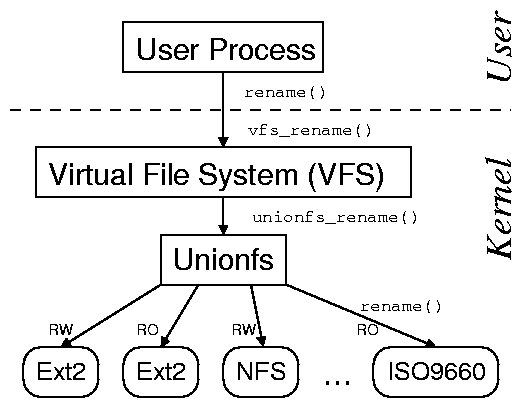
\includegraphics[width=0.4\textwidth]{chapters/background/images/unionfs.png}
	\caption[Docker \ac{ufs} overview]{Example of file renaming using the \acf{ufs}. The user's process
		see only one logical file and it is responsibility of \acf{vfs} to correctly map the rename command
		to different underlying \acf{fs}.}
	\label{img:background-docker-architecture-unionfs}
\end{figure}

\ac{ufs} uses a simple priority model which gives a unique priority to each branch . If a file exists
in multiple branches, only the copy in higher priority branch will be shown. It also allows some branches
to be read-only, but as long as at least one of them is readable and writeable, \ac{ufs} uses ``copy-on-write''
semantic to provide an illusion that all branches are writeable.

To maintain \ac{fs} integrity, Docker containers are composed by read-only layers except for the 
upper one. Another key characteristic of the Docker containers is that its \ac{fs} is designed to
be ephemeral. Then if a container contains a service that write files or data when it is running 
(like a database service), all of them will be lost after container termination. Thus in a future
launch of the same, into it we can only find the work environment (configured as described in 
the dockerfile) but without the previously generated files or data.

To ensure that this situation does not happens, there is the need to separate the container from
data life-cycle. Ideally we want that the generated data is not destroyed or tied to the container
life-cycle and can thus be reused. To achieve this, Docker provides the concepts of \keyword{data-volumes}
and \keyword{data-volumes container}.

A data-volume is a specially designed directory in the container that is able to “bypass” the \ac{ufs}.
It is initialized when the container is created and, by default, it is not deleted when the container
is stopped or when there is no container that reference it. Data-volumes are independently updated,
shareable across different containers and mountable in read-only mode too. This key feature is provided
through a symbolic link (also known as soft-link) that points to a \ac{fs} location in the \acs{os}
underlying docker daemon. Hence data will persist after container termination, and in a future launch
of it the only necessary thing to retrieve them is to fix the link (through a mount operation made at
container launch time) which point at the correct location in the underlying file-system.

Instead, a data-volume container becomes useful when we want to share data between different containers
or we want to use data from non-persistent containers. They are particular containers that aim to collect
different data-volumes and make them available for other containers.

These two features are useful when we plan to provide a backup, restore or migration features in our
applications.

\subsection{Dependency hell problem}
\label{sec:background-docker-dependencyHell}
\citeauthor{michaeljang2006} in \cite{michaeljang2006} defines the colloquial term “dependency hell” 
to point out a set of problems. It refers to the frustration problem that software developers deal with
when installing applications with dependencies on specific versions of other software packages. Modern
applications often are assembled from existing components and delegate many tasks to third parties services
and applications, so this problem must not be under-estimated.

The problem may occur in several forms: a huge number of dependencies should be downloaded and locally saved
(large amount of downloading time and storage space may be necessary), long chain of dependencies, conflicting 
dependencies, circular dependencies and finally package manager dependencies (problem encountered when 
the packet manager is not able to download linked dependencies automatically).

Docker allows to fix, implicitly, the cited problems by packaging each component and its dependencies
into a container. In particular, with Docker the following issues cannot be risen:

\begin{itemize}
	\item{\keyword{conflicting dependencies}: we can run different software versions, that require
		different dependencies or many version of them, in various containers. Each one with
		the correct one dependencies;}
	\item{\keyword{missing dependencies}: no dependency can be missing because every one is packaged
		along with the application container;}
	\item{\keyword{platform differencies}: moving from one provider to another is no longer a
		problem if both systems run the Docker daemon; the same container will execute without other
		issues.}
\end{itemize}

\subsection{Security issues}
\label{sec:background-docker-security}
Docker is becoming an interesting technology in cloud computing world and for this reason we need also
to analyse its intrinsic security issues. Speaking about Docker security, we need to focus on the following
areas: intrinsic security of Linux kernel and its support for namespaces and cgroups features, the weaknesses
of the Docker daemon itself and finally poorly configured images.

Since Docker features lie on Linux kernel, these provide an initial inherent safety. Kernel namespace
feature is the one that provides the first and straightforward form of isolation. Its main purpose is
to grant that processes inside a container cannot be seen or affected, by processes running
in other containers or in the host system. In addition each container gets its own network stack, meaning
that it cannot get a privileged access to the sockets or network interfaces of others. This means that
containers are just like physical machines connected to a common Ethernet switch, because all containers, on
a given Docker host, are placed over bridges interfaces. Cgroups are the key component of the Linux kernel
that provide resource accounting and limiting. They allow security ensuring that each container gets its fair
share of resources (memory, CPU, Disk I/O), and finally preventing a container to bring the system down due to
exhausting of computing resources. So while they do not play a role in preventing one container from accessing or
affecting data of other processes or containers, they are essential to fend off some \ac{dos} attacks, becoming
thus an interesting feature in multi-tenant environments. Both namespaces and cgroups features are available
together since Linux kernel 2.6.26 (released 8 years ago); they have been scrutinized on a large number of
production systems, so their design and their consequent implementations are pretty mature.

Running containers with Docker implies executing the Docker daemon on the host, and currently it requires
root privileges to perform its tasks. Hence only trusted system-users should be allowed to control and dialogue
with it. Docker images can request to the daemon to share directories (data-volumes) between a container
and the underlying host file-system. This means that a malicious user can start a container in which its 
``/host'' directory will be mapped to the ``/'' directory of the underlying host \acs{os}. Hence the container
will be able to alter the host file-system without restrictions while it should not have this permission.
This has a strong security implication when a cloud provider plan to provide a public \acs{api} to deploy
containers. It should be more careful than usual with the parameter checking to make sure that a malicious
user cannot pass crafted parameters causing Docker to create arbitrary containers. For this reason the Docker
REST \acs{api} endpoint is changed using, from version 0.5.2, the UNIX socket instead of a TCP bound on
127.0.0.1; This have been done because the latter are prone to \ac{csrf} attacks. Docker daemon can also be
attacked through images loading from disk or from network. This has been focus of improvements in the community,
especially for images coming from not-trusted networks. Hence from Docker 1.3.2 images are now extracted in a
chrooted sub-process on the Linux platform. In conclusion it is expected that the Docker daemon will run with
restricted privileges, delegating well-audited operations to sub-processes, each one with its own very limited
set of privileges to avoid that malicious containers can exploit vulnerabilities. This will be possible with the
future adoption of the recent improvements in Linux namespaces which includes the user-namespace. Moreover, this
will also solve the problem caused by sharing \ac{fs}s between host and guest, since the user namespace
allows users (including the root user) to be mapped to other users in the host system within containers.

Finally, many security lacks come from wrong configuration provided by the users when they define dockerfiles.
In this scenario common mistakes include software from unknown sources or wrong network configuration that
pave the way for malicious users.

%---------------------------------------------------------------------------------------------------
%		platform.tex
%
%	This file contains the sections that describe available IaaS cloud platform and its main features
%
%	Author: Andrea Meneghinello
% Version: 0.1
%	Table of changes:
%		17/03/2016 -> document definition
%---------------------------------------------------------------------------------------------------
\section{\acs{paas} cloud platforms}
\label{sec:background-cloudPlatform}
In the previous sections we have illustrated what cloud computing is and how it can make resources
available to us through the virtualization technique. 

Now we want to illustrate some of the major \ac{paas} provider competitors in the market. Each one 
has characteristics that differentiate it from the others. In the following section we will see that
some of the major competitors have started the integration of the Docker \ac{api} inside their platforms.

\subsection*{Cloud unit}
\label{sec:background-cloudPlatform-cloudUnit}
CloudUnit \cite{cloudUnitHomepage} is an open-source \ac{paas} for Java applications. It provides an
automated and standardized platform for developers to build and run Java applications, as faster as
possible, and operational to provision and orchestrate environments.

Its main characteristics are:

\begin{itemize}
	\item{\keyword{infrastructure agnostic}: it is able to run on top of any \acs{it} infrastructure
		(\ac{vm}s, bare-metal, public, private and also hybrid cloud, etc.);}
	\item{\keyword{tools}: developers can deploy new or legacy applications without changing any line
		of code and using their preferred tools;}
	\item{\keyword{portability}: it is based on Docker which ensures that deployed applications will
		work seamlessly on any environment;}
	\item{\keyword{open-source}: it is able to eliminate lock-in problem because it is licensed under
		the GNU public license 3.0.}
\end{itemize}

\subsection*{Docker data center}
\label{sec:background-cloudPlatform-dockerDataCentre}
At the end of February Docker announced \cite{dockerDataCentrePresentation} the release of its data-centre
\cite{dockerDataCentre} (shown in Figure \ref{img:background-cloudPlatform-dockerDataCetre}) which
brings containers management and services deployment to the enterprise
with a production ready \ac{caas} that is supported by Docker and hosted locally, behind their firewalls.

The biggest difference between Docker data-centre and other \ac{paas} providers is that Docker \ac{caas}
is an end-to-end fully Docker-native platform. This means that users can utilize the Docker \ac{cli}
and the full set of \acs{api}. The platform is extremely pluggable as they believe in the philosophy of
``batteries included, but swappable.'' Users can simply plug Docker \ac{caas} into their existing
environments, avoiding vendor lock-in.

\begin{figure}
	\centering{}
	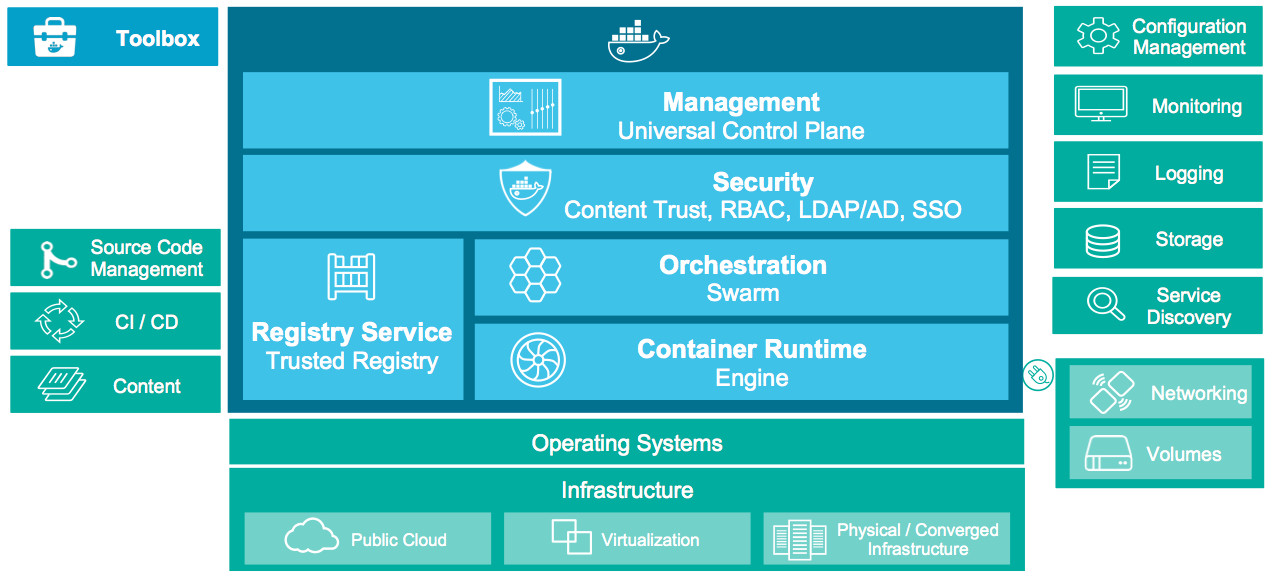
\includegraphics[width=0.75\textwidth]{chapters/background/images/docker-datacentre.png}
	\caption[Docker data-centre architecture]{Docker data-centre architecture \cite{dockerDataCentreArchitecture}.}
	\label{img:background-cloudPlatform-dockerDataCetre}
\end{figure}

\ac{paas} solutions are notorious for locking customers into using a particular infrastructure. They
are often cobbled together solutions that are not natively integrated. For instance, you could use
something like OpenShift, but then your orchestration might be Kubernetes, while also using the open
source Docker engine.

%---------------------------------------------------------------------------------------------------
%		problem.tex
%
%	This file contains the sections that describe the problem addressed in the thesis
%
%	Author: Andrea Meneghinello
% Version: 0.1
%	Table of changes:
%		11/03/2016 -> document definition
%---------------------------------------------------------------------------------------------------
\section{Problem definition}
\label{sec:problemSpace-problem}
Cloud computing is becoming more mature day by day and market has started investing on it. A recent
study, commissioned by Microsoft \cite{microsftCloudNewJob}, shows that cloud computing produces much
new innovation in \acs{it} every year:

\begin{center}
	\begin{quote}
		``Innovation created by cloud computing produce \textdollar{}1.1 trillion a year in new
		business revenues. It was also able to generate 14 million of jobs worldwide from 2011 to 2015.''
	\end{quote}
\end{center}

\ac{paas} differs from \ac{iaas} because \ac{paas} does not allow users to control the underlying
hardware. Despite all \ac{paas} advantages (described in Section \ref{sec:problemSpace-paas-paasCharacteristics})
the following issues may be still present:

\begin{itemize}
	\item{it may lead to a possible vendor lock-in if the provider imposes the use of a particular
		technology;}
	\item{it may compromise cloud resource elasticity because users are not able to configure the
		underlying hardware.}
\end{itemize}

In order for the \ac{paas} vendors to offer developers high quality services, they should use a 
virtualization layer that exploits the underlying hardware as best it can. The assets on which the
virtualization layer can make optimizations are those illustrated in Section
\ref{sec:problemSpace-paas-virtualization-assets}, hence our purpose is to compare and then analyse
classic virtualization techniques and the ones provided by the Docker framework in terms of computing,
storage and networking.

In addiction we want to find a way to obtain elasticity, without considering hardware level. Thus new
architectural patterns must be found in order to exploit elasticity offered by the cloud paradigm.

Finally we want to understand the portability value that Docker offers in order to overcome the vendor
lock-in problem.

%---------------------------------------------------------------------------------------------------
%		summary.tex
%
%	This is file contains the chapter summary.
%
%	Author: Andrea Meneghinello
% Version: 0.1
%	Table of changes:
%		21/03/2016 -> document definition
%---------------------------------------------------------------------------------------------------
\section{Summary}
\label{sec:measurements-summary}
After the execution of the tests and have analysed the collected results we can now derive some conclusion
about the two virtualization technologies: \ac{kvm} \ac{vm}s and Docker containers. 

Both are, nowadays, mature technologies that have benefited of incremental hardware and software updates.
In general, we can assert that there is, at most, a point of view that is advantageous for the hardware-virtualization
level technologies and others that are more appropriate for the \acs{os}-virtualization level ones.

If we look at the hardware performance we can observe that the Docker containers are able to exploit very well
the available underlying hardware, except for the network delay (see Section \ref{sec:measurements-network-result}).
Instead, in matter of adapt themselves to share the underlying available resources, we found that the
\ac{vm}s are more mature than the counterpart.

After working a little bit with Docker technology, we have appreciated its lightweight, the rapidity that
it follows, and the easy \acs{api} that they provide to developers. Even though the Docker container are more
recent than the \ac{kvm} \ac{vm}s, they provide to developers a good level of virtualization and make some tasks
more easier (like build environments.) We expect that in nearly future this technology will be improved and largely
preferred by many developers. 

As we asserted in the previous chapter, the only adoption of a good virtualization layer, that is able to exploit
the underlying hardware, is not sufficient to guarantee good levels of elasticity. Because of this, in the next
chapter, aware of the experience matured with the performed tests, we want to introduce a possible software
architecture that can provide good level of elasticity combined with the \acs{os}-virtualization level and that
lead developers to easily generate multi-tenants applications. 